% !TEX root = main.tex

\documentclass[runningheads]{llncs}
\usepackage{graphicx}
\usepackage{pgf}
\usepackage{pgfplots}
\usepackage{placeins}
\usepackage{float}
\usetikzlibrary{positioning}
\usepackage{underscore}
\usepackage{booktabs}
\providecommand{\mathdefault}[1]{#1}

\usepackage{amsmath}
\usepackage{enumitem}
\usepackage[english]{babel}
\usepackage{algorithm}
\usepackage{algpseudocode}
\usepackage{xcolor}
\usepackage[hidelinks]{hyperref}

\begin{document}

\title{Can Regression Tests Catch Unsafe LLM Refactorings? Behavioral Gating of Architectural Tactic Implementation}
\titlerunning{Can Regression Tests Catch Unsafe LLM Refactorings?}

\author{Anonymous Author(s)}
\authorrunning{Anonymous}
\institute{Affiliation withheld for double-blind review}

\maketitle

\begin{abstract}

Software developers increasingly rely on Large Language Models (LLMs) to restructure and improve their code automatically. This raises a basic question of trust: when an AI rewrites code, how do we know it has not quietly broken something? The natural safety net is a project's own test suite, which should fail whenever the program's behavior changes.

We built a tool that automatically improves a program's internal structure---its maintainability---by applying well-known design improvements, and that, after every change, runs the project's existing tests to confirm nothing broke. Applying it to 56 real open-source projects, we then measured whether those tests actually exercise the AI's edits. They mostly do not: in 79\% of the changed projects there was no adequate test for the edit---no suite at all, or none reaching the changed code---so a clean test run means the change was \emph{untested}, not \emph{safe}. (Where tests did cover the edit, they caught nothing, suggesting those particular changes were behavior-preserving.)

Our main finding is that, in these projects, the chief obstacle to trusting AI-driven code changes was not the AI itself but the lack of tests able to exercise its edits---suggesting automatic test generation as a necessary companion to automated refactoring.

\keywords{software testing \and regression testing \and test oracles \and generative-AI validation \and large language models \and automated refactoring \and architectural tactics \and software maintainability}

\end{abstract}

\section{Introduction}

Modern software systems spend 60--80\% of their lifecycle cost on post-deployment maintenance~\cite{bass2021software}, and developers increasingly delegate the corresponding code changes to Large Language Models (LLMs). This raises a question that is fundamentally a testing problem: when an LLM rewrites code to improve its structure, does the change preserve the program's observable behavior? The available evidence is not reassuring. DePalma et al.\ report 97.2\% behavior preservation, but that figure rests on the model's own self-evaluation; when Liu et al.\ validate comparable changes with executed unit tests, a non-trivial fraction prove unsafe~\cite{depalma2024exploring,liu2025exploring}. Shokri and Khatchadourian similarly find high syntactic correctness (95\%) but very low semantic correctness (5\%) for tactic synthesis~\cite{shokri2024ipsynth}, and large-scale studies of AI coding agents show that compilable output is routinely behaviorally wrong~\cite{horikawa2025agentic}. Generation, in short, is no longer the bottleneck---\emph{validation} is.

This bottleneck is most acute for architecture-level changes. Architectural tactics---fine-grained design decisions such as \emph{Decomposability} or \emph{Reduced Coupling} that target maintainability~\cite{bass2021software,marquez2022architectural}---by construction span multiple modules, so an incorrect edit can introduce cross-module ripple effects that local, method-level checks miss. Yet most LLM-refactoring tools never execute the project's tests, treating syntactic or self-reported success as sufficient. The natural oracle for behavior preservation is the project's own regression test suite. We therefore ask whether regression testing can serve as a behavioral safety gate for LLM-implemented architectural tactics, and we build a pipeline that selects a tactic, implements it incrementally, and gates every modification on a pre-change test baseline---rolling back on new failures and self-healing from test feedback. We evaluate it on 56 real open-source repositories, asking not only whether maintainability improves but whether existing tests can actually \emph{tell us} when an LLM change is safe.

We address the following research questions:
\begin{itemize}[nosep]
    \item \textbf{RQ1:} Can an automated LLM pipeline implement maintainability-oriented architectural tactics that measurably improve code maintainability?
    \item \textbf{RQ2:} Can regression testing act as a behavioral safety gate for these LLM-generated changes---how often does executing the project's test suite detect or prevent unsafe modifications?
    \item \textbf{RQ3:} Are existing open-source test suites adequate as behavioral oracles for architecture-level LLM changes, and how do architecture type and tactic choice affect outcomes?
\end{itemize}

The remainder of this paper is organized as follows: Section~2 reviews background and related work; Section~3 describes the methodology; Section~4 details the implementation; Section~5 presents results and discussion; Section~6 discusses threats to validity; and Section~7 concludes.

\section{Background and Related Work}

\subsection{Architectural Tactics and Quality Attributes}
Software architecture is fundamentally defined by its elements, form, and rationale~\cite{perry1992foundations}, or alternatively, as a collection of components and connectors in a specific configuration~\cite{garlan1993introduction}. Within these frameworks, \textit{architectural tactics} serve as fine-grained design decisions intended to achieve specific quality attribute responses~\cite{bass2021software}. Unlike architectural patterns (e.g., MVC, Layered), which provide broad structural templates, tactics target specific quality concerns at a finer granularity---for instance, ``Reduce Coupling'' targets modifiability, while ``Decomposability'' targets analysability and modularity. Kim et al.\ showed that quality-driven development using tactics can systematically improve targeted quality attributes when tactics are chosen from measured deficiencies~\cite{kim2009qualitydriven}.

The ISO/IEC 25010 standard~\cite{ISO25010} decomposes maintainability into five sub-characteristics: modularity, analysability, modifiability, reusability, and testability. The Maintainability Index (MI)---a composite metric combining Halstead Volume~\cite{halstead1977elements}, Cyclomatic Complexity~\cite{mccabe1976complexity}, and lines of code---has been widely adopted as a practical proxy for these sub-characteristics~\cite{oman1992maintainability}. However, its validity remains debated: Lenarduzzi et al.\ found less than 0.4\% agreement among six static analysis tools on quality issues~\cite{lenarduzzi2023critical}, highlighting the need for multi-metric evaluation.

Research by Rahmati suggests that while architectural patterns provide a structural foundation, their effectiveness is highly context-dependent; misapplication can lead to a 10\% increase in maintenance effort~\cite{rahmati2021ensuring}. M\'arquez et al.\ conducted a systematic mapping of architectural tactics in software architecture, cataloging over 40 tactics and their quality attribute impacts~\cite{marquez2022architectural}. For the purpose of this study, we refined this catalog to a subset of 32 tactics specifically focused on enhancing maintainability and modifiability, excluding those primarily targeting performance or availability. This catalog, which maps each tactic to its primary quality attribute impact (e.g., Decomposability $\rightarrow$ Analysability, Reduced Coupling $\rightarrow$ Modifiability), forms the basis for our automated tactic selection mechanism.

\subsection{LLMs in Software Refactoring}
Recent multi-agent frameworks such as MANTRA have demonstrated an 82.8\% success rate in producing compilable, test-passing refactored code through contextual RAG and multi-agent LLM collaboration~\cite{xu2025mantra}. However, empirical analysis of AI coding agents reveals a significant scale limitation: agentic refactorings are dominated by low-level, localized edits (renaming, type changes), with agents performing fewer high-level design changes than human developers~\cite{horikawa2025agentic}. This localized scope is particularly problematic for architectural tactics, which by nature require coordinated changes across multiple modules.

Research into prompt engineering indicates that while LLMs can identify up to 86.7\% of refactoring opportunities, their performance in complex tactic synthesis remains limited~\cite{liu2025exploring}. Piao et al.\ explored bridging human expertise with LLM machine understanding for refactoring, finding that structured prompts with architectural context significantly improve output quality~\cite{piao2025refactoring}. In security-related tactic implementation, Shokri and Khatchadourian found that models may achieve high syntactic correctness (95\%) but fail significantly in semantic correctness (5\%) due to an inability to coordinate inter-procedural changes across multiple classes~\cite{shokri2024ipsynth}. Martinez et al.\ conducted a systematic literature review of software refactoring with LLMs, confirming that architecture-level transformations remain an open challenge~\cite{martinez2025refactoring}.

\subsection{Test Oracles and Behavioral Validation}
Determining whether a program behaves correctly---the \emph{oracle problem}---is a long-standing challenge in software testing~\cite{barr2015oracle}. When no specified oracle exists, a project's regression suite acts as a \emph{de facto} behavioral oracle: a change is treated as safe if it leaves previously passing tests passing. This is exactly the signal we use to gate LLM edits, and its reliability depends entirely on how thoroughly the suite exercises the affected code. Where suites are weak, metamorphic testing derives oracles from necessary input--output relations~\cite{chen2018metamorphic}, and---most relevant here---LLMs can themselves synthesise tests to raise coverage: CodaMosa uses a pre-trained model to escape coverage plateaus in search-based generation~\cite{lemieux2023codamosa}, and empirical work shows LLM-generated unit tests reach competitive coverage albeit with non-trivial correctness and assertion-quality issues~\cite{schafer2024llmtest}. These techniques are complementary to our pipeline: they offer a route to the adequate oracle our results show is missing.

\subsection{Research Gaps}
The synthesis of current literature identifies three gaps that motivate this work:
\begin{itemize}[nosep]
    \item \textbf{The Validation/Oracle Void:} LLM-refactoring success is predominantly reported via self-evaluation or syntactic/compilation checks rather than executed tests~\cite{depalma2024exploring,shokri2024ipsynth,horikawa2025agentic}. Behavior preservation demands an external oracle, yet no pipeline integrates regression testing as a gate on LLM-driven architectural change, and the adequacy of existing test suites for this role is uncontrolled~\cite{liu2025exploring}.
    \item \textbf{Measurement Inconsistency:} Static analysers disagree widely---less than 0.4\% agreement among six tools~\cite{lenarduzzi2023critical}---so static metrics alone cannot confirm that a change is safe or beneficial, reinforcing the need for behavioral, test-based validation.
    \item \textbf{Implementation Void:} While methods exist for \textit{detecting} the need for tactics~\cite{marquez2022architectural} and for \textit{recovering} architectural decisions~\cite{shokri2024ipsynth}, no automated pipeline closes the loop from selection through concrete multi-file implementation to behavioral validation; the vast majority of LLM-based studies address only code-level transformations~\cite{martinez2025refactoring}.
\end{itemize}

\section{Methodology}

\subsection{Research Design}

This study evaluates whether regression testing can validate LLM-generated architectural code changes, and whether the resulting edits improve maintainability. To isolate tactic implementation from upstream error, it uses validated (manually assigned) architecture labels as input rather than LLM-inferred ones; those labels come from a separate detection study (Section~\ref{sec:eval_arch_detection}).

This study employs a quantitative pre-test/post-test experimental design. The independent variable is the application of an architectural tactic selected and implemented by an LLM, given a known repository architecture. The dependent variable is software maintainability, measured using the Maintainability Index as the primary metric. Using validated architecture labels rather than LLM-inferred classifications makes it possible to isolate the effect of tactic selection and implementation from errors introduced by the detection stage.

Each repository serves as its own control, allowing paired comparison of maintainability metrics before and after the intervention. The null hypothesis ($H_0$) is that tactic implementation does not produce a statistically significant change in the Maintainability Index. We test $H_0$ using a two-sided paired Wilcoxon signed-rank test on the 42 before/after MI pairs, with significance level $\alpha = 0.05$. The Wilcoxon test is appropriate given the small sample size ($N = 42$) and the likely non-normal distribution of $\Delta MI$. Effect size is reported as the matched-pairs rank-biserial correlation ($\hat{r}$). Bootstrap 95\% confidence intervals (10,000 resamples) for the mean $\Delta MI$ complement the hypothesis test.

\subsection{Pipeline Scope}

The pipeline (detailed in Section~\ref{sec:implementation}) comprises five phases: baseline static analysis; LLM tactic selection; iterative, test-gated tactic implementation; post-intervention static analysis; and paired statistical comparison. Repositories that fail at any phase are retained as null outcomes for failure-rate analysis.

\subsection{Dataset}

The dataset for this experiment consists of the 57 manually labeled Python backend repositories from the architecture detection study. Each repository carries a validated architectural style label (script-based, layered, or modular monolith). The use of validated labels eliminates architecture misclassification as a confounding variable and allows the evaluation to focus on tactic selection and implementation effectiveness.

\paragraph{Sampling criteria.}
Repositories were selected from an initial pool of approximately 200 Python backend projects identified through GitHub search queries combining backend-related keywords (e.g., ``flask'', ``fastapi'', ``django'', ``backend'', ``api'') with minimum 10 stars and at least 5 Python files. Inclusion criteria required: (a) the repository implements a backend service or API (excluding CLI tools, libraries, and educational projects); (b) at least one Python file contains a class or function definition (excluding pure configuration or test-only repositories); (c) the repository is publicly accessible. After applying these filters, 57 repositories were retained and manually labeled for architecture style.

One repository was unavailable at run time, leaving 56, of which 42 produced paired before/after measurements; the 14 failures are broken down in Table~\ref{tab:exp5_outcomes}.

\subsection{Maintainability Measurement}

The primary metric is the Maintainability Index (MI), computed using Radon~\cite{oman1992maintainability} as a weighted composite of Halstead Volume~\cite{halstead1977elements}, Cyclomatic Complexity~\cite{mccabe1976complexity}, and lines of code, aligned with the ISO/IEC 25010 quality model~\cite{ISO25010}. Maintainability change is quantified as:

\begin{equation}
\Delta MI = MI_{after} - MI_{before}
\end{equation}

Repositories are classified as \textit{improved} ($\Delta MI > 0.01$), \textit{stable} ($|\Delta MI| \le 0.01$), or \textit{worsened} ($\Delta MI < -0.01$); the $0.01$-point tolerance treats sub-rounding differences as no-ops. Structural metrics including fan-out and docstring coverage are collected as supplementary indicators.

\subsection{Tactic Catalog}

Tactic selection is grounded in the catalog established by Bass et al.~\cite{bass2021software} and mapped by M\'arquez et al.~\cite{marquez2022architectural}. Three maintainability-oriented tactics were applied:

\begin{itemize}[nosep]
    \item \textbf{Decomposability:} splitting monolithic modules into smaller cohesive units to improve analysability;
    \item \textbf{Localized Modification:} encapsulating change-prone logic to reduce ripple effects;
    \item \textbf{Reduced Coupling:} introducing abstraction or mediators to minimize inter-module dependencies.
\end{itemize}

\subsection{Model Configuration}

All LLM calls use \texttt{Qwen3-Coder-34B} (HuggingFace: \texttt{Qwen/Qwen3-Coder-34B-Instruct}) via the Ollama API with temperature 0.2, top-p 0.9, repetition penalty 1.1, and a 256k-token context window, giving the model a repository-wide view for reasoning about cross-module dependencies~\cite{piao2025refactoring}. Tactic selection and the test-gated implementation loop---including how each accepted change is checked against the repository's tests for regressions---are detailed in Section~\ref{sec:implementation}.

\subsection{Prior Stages and Baseline}
\label{sec:eval_arch_detection}

The architecture-detection stage was evaluated separately on the same 57 repositories (separate dataset~\cite{anon_archdetect_2026}); the LLM detector reached 86.0\% accuracy (49/57) against manual labels, and we use those validated labels here to remove detection error as a confounder. A prior run of the same pipeline with \emph{LLM-inferred} labels achieved only an 18.2\% improvement rate (mean $\Delta MI = +0.48$); the present study, with validated labels, reaches 42.9\%---consistent with, though not proof of, fewer tactic-selection errors, since the datasets also differ.

\FloatBarrier
\section{Implementation}
\label{sec:implementation}

This section describes the implementation of the automated pipeline that connects tactic selection to code modification. The pipeline is implemented in Python (767 lines of core logic across five filter modules) and follows the Pipes and Filters architectural style~\cite{bass2021software}, where each stage is an independent filter that reads artifacts produced by the previous stage and writes its own outputs as JSON files on disk. This design enables stage-level fault isolation, independent execution, and incremental debugging.

Figure~\ref{fig:pipeline_arch} illustrates the overall data flow.

\begin{figure}[H]
\centering
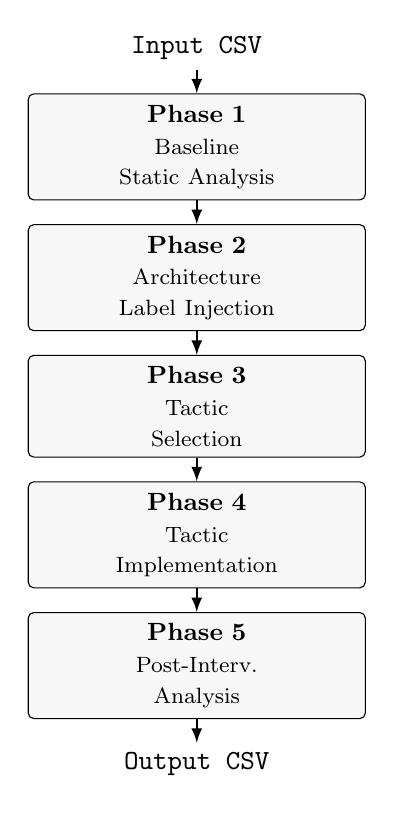
\begin{tikzpicture}[>=latex, font=\small,
  box/.style={draw, rectangle, rounded corners=2pt, text width=4cm,
              align=center, inner sep=4pt, fill=black!3},
  arr/.style={-latex, thick}]

\node[font=\ttfamily] (in) {Input CSV};
\node[box, below=0.3cm of in] (p1) {\textbf{Phase 1}\\[2pt] \footnotesize Baseline\\ Static Analysis};
\draw[arr] (in) -- (p1);

\node[box, below=0.3cm of p1] (p2) {\textbf{Phase 2}\\[2pt] \footnotesize Architecture\\ Label Injection};
\draw[arr] (p1) -- (p2);

\node[box, below=0.3cm of p2] (p3) {\textbf{Phase 3}\\[2pt] \footnotesize Tactic\\ Selection};
\draw[arr] (p2) -- (p3);

\node[box, below=0.3cm of p3] (p4) {\textbf{Phase 4}\\[2pt] \footnotesize Tactic\\ Implementation};
\draw[arr] (p3) -- (p4);

\node[box, below=0.3cm of p4] (p5) {\textbf{Phase 5}\\[2pt] \footnotesize Post-Interv.\\ Analysis};
\draw[arr] (p4) -- (p5);

\node[font=\ttfamily, below=0.3cm of p5] (out) {Output CSV};
\draw[arr] (p5) -- (out);
\end{tikzpicture}
\caption{Pipeline architecture and artifact flow (Pipes and Filters style). Artifacts are stored as JSON files at each phase.}
\label{fig:pipeline_arch}
\end{figure}

\subsection{Phase 1: Baseline Static Analysis}

The \texttt{StaticAnalysisFilter} runs the Radon tool to compute the Maintainability Index (MI) for every Python file in the repository. In addition to MI, it collects architecture-level proxies: package count, package hierarchy depth, import graph density, and file-level fan-out. Docstring coverage is computed as the ratio of functions and classes with docstrings to the total. All metrics are written into per-repository JSON artifacts under \texttt{static\_analysis/BEFORE/\{repo\}/}.

\subsection{Phase 2: Architecture Label Injection}

Validated architecture labels from the dataset (script-based, layered, or modular monolith) are injected as JSON artifacts with confidence 1.0 and evidence set to \texttt{"Pre-computed in dataset (manual label)"}. This step replaces the automated architecture detection stage, whose evaluation data are available as a separate dataset~\cite{anon_archdetect_2026}; using ground-truth labels eliminates architecture misclassification as a confounding variable in the evaluation of tactic selection and implementation.

\subsection{Phase 3: Tactic Selection}
\label{sec:impl_tactic_selection}

The \texttt{ArchitectureTacticSelectionFilter} calls \texttt{Qwen3-Coder-34B} via the Ollama API with the following context:
\begin{itemize}[nosep]
    \item Validated architecture type and confidence;
    \item Per-file static analysis metrics (MI, cyclomatic complexity, Halstead Volume);
    \item Repository file tree in ASCII form (rendered by \texttt{build\_repo\_tree});
    \item Python file signatures: imports, class names, and function signatures extracted by \texttt{extract\_python\_signatures}.
\end{itemize}

Acting as a senior software architect, the model selects the single most appropriate tactic from a catalogue of 32 maintainability-oriented tactics derived from~\cite{marquez2022architectural} and returns a structured JSON object (the selected tactic with its quality-attribute impact, a justification, target components, an implementation strategy, and risks). If no tactic applies, it returns \texttt{(none)} and the repository is excluded from implementation.

\subsection{Phase 4: Tactic Implementation}
\label{sec:impl_tactic_implementation}

The \texttt{ArchitecturalTacticImplementationAgent} applies the selected tactic through an iterative planner loop (up to ten iterations per repository). Every Python file is first parsed with \texttt{ast} into a compact index (imports, classes, functions, size) that summarises the codebase within the model's context window and feeds BM25 relevance ranking ($k_1{=}1.5$, $b{=}0.75$); the five most relevant files for the tactic are offered to the model as candidates. At each iteration the model selects one file (or \texttt{STOP}) and proposes a single change as JSON (\texttt{modify\_file}/\texttt{create\_file}, with path and content); four consecutive invalid plans abort the repository.

\paragraph{Behavioral gating.}
This is the safety mechanism at the heart of our study. Before any change, the pipeline detects pytest infrastructure (\texttt{pytest.ini}, \texttt{pyproject.toml}, \texttt{setup.cfg}, or a \texttt{tests/} directory) and, if present, records a baseline run of \texttt{pytest -q --tb=line -rf --no-header} (300\,s timeout): the set of pre-existing failures. Each proposed change is validated (non-empty, not \texttt{\_\_init\_\_.py}, $\leq$400 lines), the target file is snapshotted, the patch is applied, and pytest is re-run. If failures appear that were absent from the baseline---a regression---the file is restored and up to two \emph{self-healing} attempts feed the failing test output back to the model for a minimal, behavior-preserving fix; if these fail, the step is abandoned. Repositories without tests skip gating, with the baseline treated as trivially passing. The full prompt templates and planner pseudocode are provided in the replication package.

\subsection{Phase 5: Post-Intervention Analysis}

After the implementation phase, \texttt{StaticAnalysisFilter} re-runs on the modified codebase. Results go to the \texttt{AFTER} artifact directory. The change $\Delta MI = MI_{after} - MI_{before}$ is computed per file and for the repo average.

A summary of all outcomes (improved, stable, worsened, or failed) is appended to the output CSV along with the architecture label and chosen tactic name. Repositories that fail at any phase (clone failure, tactic selection failure, planner failure) are recorded as null outcomes and retained in the dataset for failure rate analysis.

\section{Results and Discussion}

\subsection{Overall Quantitative Impact}

Of 56 repositories (Table~\ref{tab:exp5_outcomes}), 14 (25.0\%) failed---10 during cloning, 4 during implementation---leaving 42 with paired measurements, of which 18 improved, 17 were stable, and 7 worsened. We report two rates throughout: the per-protocol rate (18/42 = 42.9\% of completed) and the intention-to-treat rate (18/56 = 32.1\% of all), the realistic end-to-end success rate including infrastructure and planning failures.

\begin{table}[H]
\centering
\small
\caption{Pipeline outcome distribution (N = 56).}
\label{tab:exp5_outcomes}
\begin{tabular}{lrr}
\toprule
\textbf{Outcome} & \textbf{N} & \textbf{Share} \\
\midrule
Improved ($\Delta MI > 0.01$)  & 18 & 42.9\% of completed (32.1\% of all) \\
Stable ($|\Delta MI| \le 0.01$)    & 17 & 40.5\% of completed \\
\quad Syntax error          & 3  & 7.1\% of completed \\
\quad Planner failure       & 7  & 16.7\% of completed \\
\quad No-op modification    & 7  & 16.7\% of completed \\
Worsened ($\Delta MI < -0.01$)  & 7  & 16.7\% of completed \\
Failed / null               & 14 & 25.0\% of all \\
\midrule
\textbf{Total} & \textbf{56} & \\
\bottomrule
\end{tabular}
\end{table}

As Table~\ref{tab:exp5_outcomes} shows, the ``stable'' category is heterogeneous: only 7 of 17 are genuine no-op edits, while 7 are planner failures and 3 are syntax errors where no valid change was made. Counting only the 32 cases where code was actually modified, the improvement rate is 56.2\% (18/32).

Descriptive statistics for the 42 completed repositories are shown in Table~\ref{tab:exp5_mi}.

\begin{table}[H]
\centering
\small
\caption{Maintainability Index statistics for completed repositories (N = 42).}
\label{tab:exp5_mi}
\begin{tabular}{lr}
\toprule
\textbf{Metric} & \textbf{Value} \\
\midrule
Mean $\Delta MI$ (all completed)  & +1.484 \\
Mean $\Delta MI$ (improved only)  & +3.716 \\
Mean $\Delta MI$ (worsened only)  & $-$0.653 \\
\bottomrule
\end{tabular}
\end{table}

Both the improvement rate and the mean gain exceed the initial pipeline experiment (Section~\ref{sec:eval_arch_detection}; 18.2\%, +0.48)---consistent with, but not proof of, better tactic selection from validated labels, since the datasets also differ.

\subsection{Behavioral Gating and Test Adequacy}
\label{subsec:exp5_testing}

Because behavioral validation is this paper's primary question, we address it (RQ2, RQ3) before the detailed maintainability analysis (RQ1). After every accepted modification the pipeline re-ran the repository's test suite against a pre-change baseline (Section~\ref{sec:impl_tactic_implementation}). The planner applied changes to 28 of the 42 completed repositories (208 steps); across the per-step logs the regression gate never triggered---not one step introduced a new test failure.

Across those 121 logged steps the regression gate never triggered: not one introduced a new test failure relative to baseline. To learn whether that null is meaningful, we measured both the gate and the suites directly (replication package, \texttt{measure\_edit\_coverage.py}). A \emph{positive control}---a seeded behavior-changing mutation injected into a covered line of an edited file---made the affected suite fail, confirming the gate detects regressions when tests reach the changed code. We then re-ran each suite under coverage instrumentation to measure how much of the LLM-edited code the existing tests exercise. This exposes why the gate stayed silent: of the 28 modified repositories, \textbf{15 (54\%) had no test suite at all}; of the 13 with tests, five changed only newly-created files (uncovered by pre-existing tests by construction), and among the eight that edited existing files the median coverage of those files was only 38\% (range 0--85\%, two at 0\%). In total, \textbf{22 of 28 repositories (79\%) had no adequate oracle for the change the LLM made}.

This disaggregates the silent gate into its real causes. In 79\% of cases the gate was effectively blind---no tests, untested new files, or uncovered lines---so there a passing gate means \emph{untested}, not \emph{validated}: a quantified \emph{test-adequacy gap}. In the remaining six repositories the tests \emph{did} exercise the edited code (coverage up to 85\%) yet still flagged nothing---the opposite signal, indicating those particular edits were most likely behavior-preserving. The headline ``zero regressions'' is therefore neither vindication nor pure artifact but a mixture: predominantly the absence of an oracle, occasionally genuine preservation. The practical consequence for architecture-level LLM changes is that an existing suite is usually too thin to act as a behavioral oracle; pairing LLM refactoring with LLM-assisted test generation~\cite{cordeiro2024llm,schafer2024llmtest}---ideally coverage-driven~\cite{lemieux2023codamosa}---to synthesise an adequate oracle before trusting the gate is the natural next step. Either way, the compile-or-self-evaluate success criteria common in prior work~\cite{depalma2024exploring,horikawa2025agentic} substantially overstate safety.

\subsection{Inferential Statistics}

We tested $H_0$ (median $\Delta MI = 0$) with a two-sided paired Wilcoxon signed-rank test on the 42 pairs (differences within the $\pm0.01$ tolerance treated as ties). The result is significant ($W = 81$, $p = 0.028$, matched-pairs rank-biserial $\hat{r} = 0.50$; 95\% bootstrap CI for the mean $\Delta MI$ [0.29, 2.98], 10{,}000 resamples)---a non-trivial effect, but one concentrated in a subset of repositories.

\paragraph{Sensitivity analysis.}
The two largest improvements---webapp-color ($\Delta MI = +21.98$) and Paper2Rebuttal ($\Delta MI = +18.14$)---exert disproportionate influence. Removing both, the mean $\Delta MI$ drops from +1.48 to +0.56 and the Wilcoxon test is no longer significant ($p = 0.083$). The overall positive result is thus not uniform: it is driven by a few high-impact cases, primarily small repositories where file splitting mechanically inflates MI. Most repositories (26/42, 61.9\%) show $\Delta MI$ within $\pm 0.5$ points, indistinguishable from measurement noise.

These analyses use a per-protocol sample ($N = 42$). Because the Wilcoxon test discards zero-difference pairs, treating the 14 failures as $\Delta MI = 0$ leaves the statistic unchanged; the realistic intention-to-treat picture is conveyed instead by the success rate of 18/56 (32.1\%)---a real but modest effect.

\subsection{Notable Improvement Cases}
\label{subsec:exp5_cases}

To understand \textit{how} the pipeline produced MI gains, we examined the largest improvements; two contrasting cases capture the dominant mechanism---extracting new cohesive modules from files with low or near-zero MI.

\paragraph{webapp-color ($\Delta MI = +21.98$, Decomposability).}
A single-file Flask app (\texttt{app.py}, MI = 69.27) was split into a revised \texttt{app.py} (MI = 73.74) plus \texttt{color.py} and \texttt{config.py} (both MI = 100), raising the average to 91.25. This is the idealized---but also the most superficial---case: the gain is largely an artifact of small size, where each trivial new file carries equal weight.

\paragraph{Paper2Rebuttal ($\Delta MI = +18.14$, Localized Modification).}
Here \texttt{rebuttal\_service.py} had MI = 0.0 (Radon rank C). The model recognised that it mixed PDF conversion, LLM orchestration, and arXiv access, and extracted three dedicated modules (MI = 61.6, 50.1, 34.8); the original file rose to MI = 55.6. Unlike webapp-color, this reflects a genuine separation of responsibilities---yet MI alone cannot distinguish the two.

\paragraph{Common pattern.}
Across the dataset, 12 of 18 improvements extracted a new module scoring MI = 100 (configuration objects, pure utilities, simple API clients) and four others partially relieved an MI = 0 file (the remaining two combined smaller code-level edits). All raise the repository average through the non-linear MI formula more than through real architectural restructuring.

\subsection{Results by Architectural Tactic}

Table~\ref{tab:exp5_tactics} shows outcomes grouped by selected tactic.

\begin{table}[H]
\centering
\small
\caption{Results by architectural tactic.}
\label{tab:exp5_tactics}
\begin{tabular}{lrrrrl}
\toprule
\textbf{Tactic} & \textbf{N} & \textbf{Impr.} & \textbf{Stable} & \textbf{Worse.} & $\overline{\Delta MI}$ \\
\midrule
(none selected)       & 7  & 0 & 7 & 0 & 0.00  \\
Decomposability       & 18 & 8 & 7 & 3 & +2.33 \\
Localized Modification & 14 & 9 & 3 & 2 & +1.49 \\
Reduced Coupling      & 3  & 1 & 0 & 2 & $-$0.16 \\
\bottomrule
\end{tabular}
\end{table}

\textbf{Localized Modification} has the best risk-adjusted profile (9 improvements, 2 worsenings; mean +1.49): it encapsulates change-prone logic without creating new, possibly below-average modules. \textbf{Decomposability} yields the largest individual gains but the most worsenings---high variance, since extracted files can sit below the repository average. \textbf{Reduced Coupling} (only 3 cases) never improved MI, with 2 of 3 worsening.

\subsection{Results by Architectural Style}

Table~\ref{tab:exp5_arch} presents results grouped by validated architecture label.

\begin{table}[H]
\centering
\small
\caption{Results by architectural style.}
\label{tab:exp5_arch}
\begin{tabular}{lrrrrr}
\toprule
\textbf{Architecture} & \textbf{N} & \textbf{Impr.} & \textbf{Worse.} & \textbf{Stable} & $\overline{\Delta MI}$ \\
\midrule
Script-based      & 7  & 3 & 0 & 4 & +5.62 \\
Modular monolith  & 26 & 9 & 5 & 12 & +0.76 \\
Layered           & 9  & 6 & 2 & 1  & +0.35 \\
\bottomrule
\end{tabular}
\end{table}

\textbf{Script-based} repos improve most (+5.62): few files, low-MI monolithic scripts, clear decomposition targets. \textbf{Modular monoliths} (+0.76) account for all five worsenings---already-organized code is sensitive to restructuring. \textbf{Layered} repos improve most often (6/9) but only modestly (+0.35), as explicit layers give tactic application a cleaner target.

\subsection{Supplementary Architectural Metrics}

MI is insensitive to inter-module structure, so we also report three architecture-level metrics---average fan-out, package count, and maximum directory depth (Table~\ref{tab:exp5_supp}).

\begin{table}[H]
\centering
\small
\caption{Supplementary architecture-level metric changes (N = 42).}
\label{tab:exp5_supp}
\begin{tabular}{lrrr}
\toprule
\textbf{Metric} & \textbf{Before} & \textbf{After} & \textbf{$\Delta$} \\
\midrule
Mean avg.\ fan-out        & 4.12 & 3.95 & $-$0.17 \\
Mean package count        & 9.7  & 9.7  & 0.00 \\
Mean max.\ directory depth & 2.4  & 2.4  & 0.00 \\
\bottomrule
\end{tabular}
\end{table}

Package count and directory depth were unchanged across all 42 repositories, and fan-out moved only marginally ($-$0.17, from four repositories where new files absorbed imports). The pipeline thus operates at the code level (splitting files, extracting functions), not the architecture level (reorganizing packages or introducing layers); even Paper2Rebuttal---the one case with a notable fan-out drop ($-$2.1)---left the package structure intact. This is why we treat MI gains cautiously and foreground the behavioral question instead.

\subsection{Stable and Worsened Outcomes}

The 17 stable outcomes comprise 7 genuine no-op edits (docstrings or import reordering, which do not affect MI), 7 planner failures, and 3 syntax errors (Radon excludes the malformed file). The seven worsening cases all extracted a module scoring below the repository average; the worst was only $-1.23$ MI (\textit{geo-seo-claude}), and all fell within the tiny or small size bins.

\subsection{Pipeline Failure Analysis}

The 14 failed cases divide into two categories: infrastructure failures (10 repositories lost during cloning due to repository deletion, privatization, or access restrictions) and algorithmic failures (4 repositories with completed before-analysis but no after-analysis measurements due to planner or API issues).

\paragraph{Failed vs.\ completed comparison.}
To check for attrition bias, we compared the 14 failed and 42 completed repositories on available covariates: median file count (13.5 vs.\ 17.5), architecture-type distribution, and baseline MI were all similar. The sample is too small for a formal test, but the differences are not large enough to indicate strong selection bias.

Implementation-stage failures mixed infrastructure issues (HTTP 429 rate limiting) with algorithmic ones (malformed planner JSON, a stuck regeneration loop, invalid file paths). The distinction matters: infrastructure failures are mitigable with retry strategies, whereas algorithmic failures require fundamental improvements in LLM planning.

\subsection{Discussion}

\paragraph{What the MI gains really mean.} Effect magnitude is dominated by repository size: medium and large repos show median $|\Delta MI|$ of 0.05 and 0.00---noise---so the pipeline yields measurable gains only on small repos with a clearly separable concern. Even there, the gain is largely metric arithmetic: a new MI = 100 file raises a one-file repo's average by $\approx$15 points regardless of architectural merit, and removing the two outliers erases statistical significance ($p = 0.083$). With package structure and fan-out essentially unchanged (Table~\ref{tab:exp5_supp}), MI improvement is at best a weak proxy for architectural improvement.

\paragraph{Why this matters for testing.} The more robust result is the validation gap (Section~\ref{subsec:exp5_testing}): the regression gate could not confirm safety because the test suites were inadequate. An MI gain that is simultaneously a metric artifact \emph{and} unverified by tests is doubly untrustworthy---reinforcing that automated refactoring needs a behavioral oracle, not merely a quality metric.

\paragraph{Implications for practice.} (i) Apply the pipeline only to small repositories ($<$30 files), and expect a realistic $\sim$32\% end-to-end success rate. (ii) Prefer Localized Modification; avoid Reduced Coupling, which produced no positive outcomes. (iii) Never equate an MI gain---or a passing run of a sparse test suite---with a safe, architectural improvement; validate with an adequate test suite, generating one if necessary. (iv) The planner is brittle; structured or constrained decoding would improve reliability over free-form JSON.

\section{Threats to Validity}

\textbf{Internal validity.} Labels came from a single annotator (no inter-rater check). Because the largest gains arise from MI = 0 files, part of the effect may be regression to the mean rather than tactic effectiveness; a ``do-nothing''/random-split control (future work) would quantify the background rate. A single model was used.

\textbf{External validity.} The 56 repositories are open-source Python backends in three architectural styles; results may not transfer to other languages, industrial code, or larger systems.

\textbf{Construct validity.} MI measures file-level complexity, not module-boundary quality or coupling, so it cannot in principle capture the effect of \texttt{Reduced Coupling}. For behavioral validation, our coverage measurement (Section~\ref{subsec:exp5_testing}) used best-effort dependency installation; suites that failed to install fully would under-report coverage, which if anything strengthens the test-adequacy finding. Behavior preservation is confirmed only for the minority of edits the suites actually cover; for the 79\% without an adequate oracle it remains unverified.

\textbf{Conclusion validity.} The sample is small (42 completed, 18 improvements); significance vanishes when the two outliers are removed ($p = 0.083$), and subgroup analyses (e.g., \texttt{Reduced Coupling}, $N=3$) have little power. Results are early feasibility evidence, not definitive performance claims.


\section{Conclusion}
\label{sec:conclusion}

This paper studied regression testing as a behavioral safety gate for LLM-driven architectural change. An LLM pipeline (Qwen3-Coder-34B) selected and implemented maintainability tactics on 56 open-source Python projects, gating every edit on the project's existing tests.

Two results stand out. The maintainability gains were real but fragile: a Wilcoxon test on 42 before/after pairs was significant ($p = 0.028$, $\hat{r} = 0.50$) yet fell to non-significance once two outliers were removed ($p = 0.083$); gains concentrated in tiny repositories, and package structure and fan-out were unchanged---so the pipeline operates at the code level, not the architecture level. More importantly, we measured whether the gate could validate the changes at all: a seeded-fault positive control confirmed it fires, but in 79\% of modified repositories no adequate test existed (no suite, new files, or uncovered code), so the zero-regression result reflects missing oracles far more than verified safety---though where tests did cover an edit, none failed.

In our sample, the binding constraint on trustworthy AI refactoring was the absence of adequate test oracles, not generation capability. The clearest next step is to pair the pipeline with LLM-assisted test generation that synthesises an oracle before gating; further work includes multi-model comparison, file- and module-level metrics for larger repositories, and more robust (structured-decoding) planning.

\begin{credits}
\subsubsection{\ackname}
The authors declare the use of AI tools in the preparation of this manuscript: Qwen3-Coder-34B was used for code generation in the experimental pipeline; Claude (Anthropic) was used for writing assistance and \LaTeX{} formatting.

\subsubsection{Disclosure of Interests}
The authors have no competing interests to declare.
\end{credits}

\section*{Data Availability}

The replication package---the LLM prompt templates, pipeline source, per-repository static-analysis artifacts (Radon MI logs, architecture proxies) and per-step test/gating records, the outcome dataset, and the behavioral-validation experiment (\texttt{measure\_edit\_coverage.py} with its coverage and positive-control results)---is available in an anonymized repository for double-blind review at \url{https://osf.io/yn4h6/?view_only=0780faf0988448e2ba1667a2fcc53678}, and will be deposited in a public archive with a DOI upon acceptance. The experimental model is \texttt{Qwen/Qwen3-Coder-34B-Instruct} (HuggingFace); all non-default generation parameters are included in the package.
\bibliographystyle{splncs04}
\bibliography{ref}

\end{document}